As discussed in the preceding, the translation from high-level neural network specification to hardware native involves a diverse set of choices at design time and translation time.
Any such choice made implicitly by the DL framework abstracts away intermediary details at the level of abstraction at which the choice is made.
For example, in PyTorch, by default convolutions include not only learnable filters but also a learnable bias.
Naturally this increases the number of parameters for which gradients need to be kept account of and updated for.
At the next level of abstraction (translation from Python specification to C++ objects) another implicit choice is made in choosing tensor dimension ordering%
\footnote{PyTorch uses some heuristics to order tensor dimensions either NCHW or NHWC.}.
Finally, at the level of abstraction just prior to compilation into CUDA kernels a convolution strategy is chosen%
\footnote{Winograd convolution, general matrix multiply (GEMM), or FFT convolution.} according to heuristics.
Each of these choices potentially incurs a runtime execution and memory cost, depending on whether the heuristics according to which the choice was made apply to the DL model.

With this as subtext, we describe the intent and design of our experiments.
We implement the popular object detection deep neural network ResNet-50~\cite{he2015deep} at four levels of abstraction (PyTorch, TorchScript\footnote{TorchScript models are serializations of PyTorch models but can run in inference mode in C++, i.e. sans Python runtime.}, LibTorch, and cuDNN) in order to investigate the differences amongst them.
We measure accuracy, execution time, GPU utilization, and memory efficiency of each implementation on four image datasets (MNIST, CIFAR10, STL10, PASCAL).
The source for the implementations is available on GitHub\footnote{\url{https://github.com/makslevental/pytorch_abstraction_comparison}}.
The datasets were chosen because they span the spectrum of image complexity (from small single-channel to large multi-channel).
The reasons for choosing ResNet-50 (see~\cref{fig:resnet}) are two fold.
Firstly, it serves as a benchmark architecture in the research community.
Secondly, it includes functional units included in many other network architectures (residual units, convolutions of various sizes, batch normalizations, ReLU activations, and pooling layers) and is therefore representative of typical neural network compute workloads.
The reason for staying within the same ecosystem is that, in theory, we fix as many of the dimensions of functionality orthogonal to our concerns as possible.

\begin{figure}
    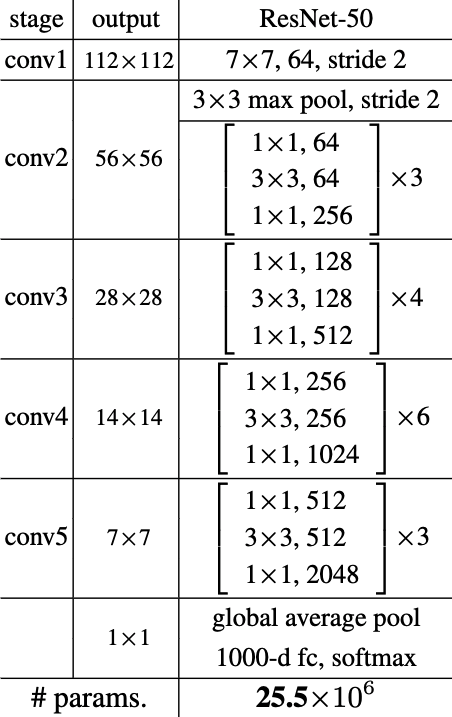
\includegraphics[width=.6\linewidth]{figures/resnet50.png}
    \caption{ResNet-50 network architecture~\cite{he2015deep}.}
    \label{fig:resnet}
\end{figure}


We employ two test platforms (see~\cref{tab:platforms});
training is performed for 100 epochs with batch size 128 (except for on PASCAL where we use batch size 16) on the ``Training platform''.
Distinct models were trained in parallel in order to expedite the overall training process but neither data parallelism nor intra-model parallelism were employed.
In addition we perform scaling experiments (in resolution and batch size) on the PASCAL dataset;
for $\code{batch\_size}, \code{resolution} = 8, 16, \dots, 1024$.
For this purpose we employ the ``Resolutions platform'', which has GPU RAM enough to accommodate large batch sizes and large image resolutions.
For both sets of experiments, each run is repeated 10 times to reduce variance in the measurements.
Precise execution time measurements are collected using the CUDA \code{cudaEventCreate}, \code{cudaEventRecord}, \code{cudaEventElapsedTime} APIs.
Precise memory and GPU utilization measurements are collecting using the NVIDIA Management Library C API\@.
Both sets of APIs were appropriately wrapped for use in Python.

\begin{table}
  \caption{Test platforms}
%  \vspace{-2ex}
  \centering
  \begin{tabular}[t]{p{0.15\linewidth}p{0.75\linewidth}}
    \hline
    CPU      & AMD Ryzen 2970WX 24-Core @ 4.2 GHz                              \\
    GPU      & 4 $\times$ GeForce GTX 1080Ti                                              \\
    HD       & Crucial MX500 2TB 3D NAND SATA                                  \\
    RAM      & 64GB                                                            \\
    Software & PyTorch-1.7.0, CUDA-11.1, NVIDIA-455.23.05, g++10.1.0           \\
    \hline
  \end{tabular}
  \subcaption*{Training platform}
  \bigskip
  \begin{tabular}[t]{p{0.15\linewidth}p{0.75\linewidth}}
    \hline
    CPU      & Intel Xeon Gold 6230 CPU @ 2.10GHz                              \\
    GPU      & Tesla V100-PCIE-32GB                                            \\
    HD       & HPE 800GB SAS 12G Mixed Use SFF                                 \\
    RAM      & 384GB                                                           \\
    Software & PyTorch-1.7.0, CUDA-11.1, NVIDIA-450.80.02                      \\
    \hline
  \end{tabular}
  \subcaption*{Resolutions platform}\label{tab:platforms}
\end{table}


